
\section{【京大に機動隊が!?】僕の熊野寮ガサ体験記}\label{sec:gasataiken}

\bunsekisha{文責}{雨蛙}

\begin{figure}[h]
  \centering
  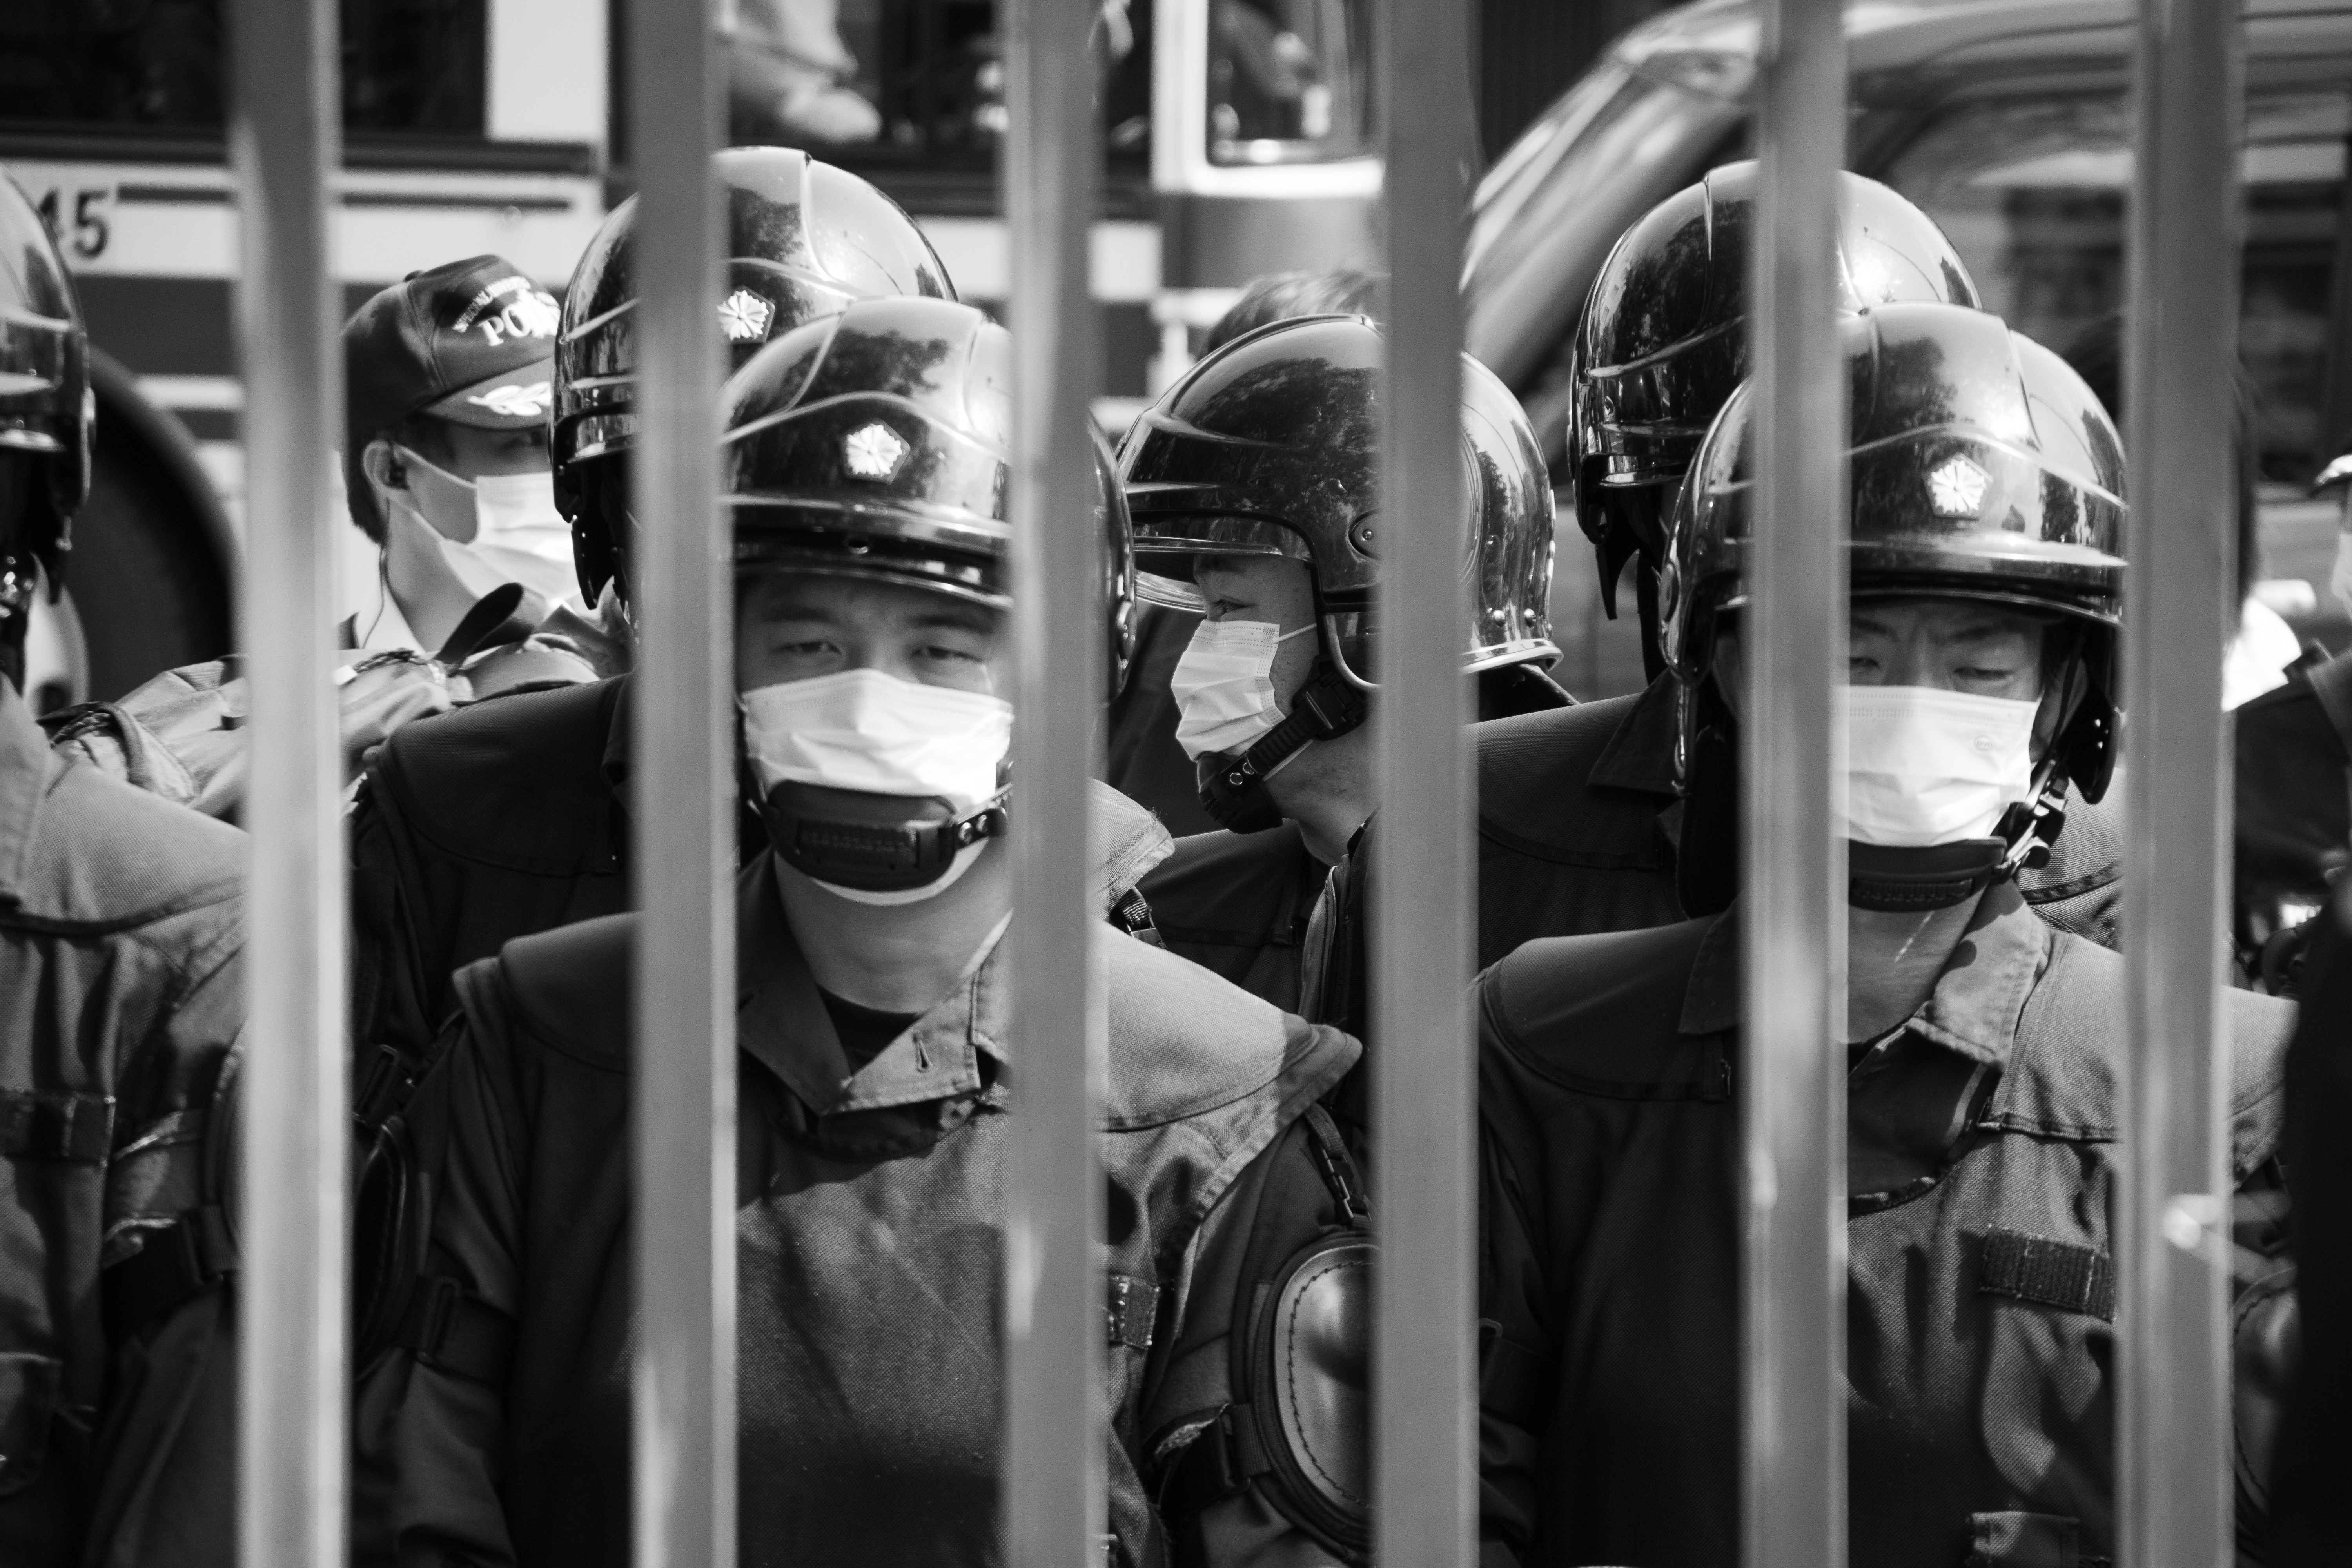
\includegraphics[width=10cm]{gazo/kidotai.jpg}
  \caption*{{\small 封鎖された正門前に並ぶ機動隊}}
\end{figure}



熊野寮生の雨蛙と言います。去る2021年6月24日、僕は初めて自分の家に家宅捜索(いわゆる「ガサ」)が入るという経験をしました(捜索対象は僕の部屋ではなかったですが)。ツイッターではひとしきり盛り上がりましたし、テレビで全国ニュースとして取り上げられたりもしたので、ご存知の方は多いと思います。

この記事はいち熊野寮生の立場から、このガサがどのように見えたのかを書いたものです。ガサのニュースを見て「熊野寮やべーな」と感じた人は多いと思いますが、僕の実感はむしろ逆で「警察やべーな」です。「そんなん熊野寮生の一方的な見方やろ」という声が飛んできそうですが、この記事を読めば、きっとあなたも「警察やべーな」ってなります。

「警察やべーな」ポイントはいくつかあります。

\begin{itemize}
  \item 思想差別的なチョー微罪逮捕がやばい!
  \item 証拠があるとは思えない熊野寮に捜索に来るのがやばい!
  \item メディアを引き連れて、熊野寮を撮影するのがやばい!
  \item 寮生は捜索妨害しないのに機動隊200人連れてくるのがやばい!
  \item 令状もないのに寮生の部屋を覗いたり、バイクのナンバーをメモってるのがやばい!
  \item 実際押収品は寮生のノートたったの一冊!
  \item 熊野寮のネガキャンがしたいだけで草!
\end{itemize}

という感じです。順次説明していきますね。

\noindent *この記事は、あくまでいち熊野寮生としてガサについてどう思っているのかを書いたもので、寮生全員が同じような感想を持っているとは限りませんし、熊野寮自治会の立場でもありません。寮自治会のガサについての立場は熊野寮ホームページから声明「2021年6月24日家宅捜索に関する抗議声明」、あるいは本パンフレットのp.\pageref{sec:gasa_jiti}を参照してください。

\subsection{Aさん逮捕}

今回の捜索は、中核派の活動家であるAさんの逮捕に関連するものです。僕が把握している時系列はこんな感じです。

\begin{itemize}
  \item 6月21日午前 Aさん逮捕
  \item 同日午後 Aさんの京都の\textbf{下宿}などに家宅捜索
  \item 6月23日 Aさんの勾留延長が決定
  \item 6月24日9時ころ Aさんの立ち回り先として\textbf{熊野寮}に家宅捜索
  \item 7月1日 Aさん勾留満期で釈放
\end{itemize}

逮捕容疑は「免状不実記載」、つまり「免許証の更新時に居住実態のある京都の下宿ではなく、実家の住所を書いた」というものでした(誤解が多いかもしれませんが、\textbf{Aさんは寮に住んでいたわけではない}です。寮とは別にAさんの下宿とされるアパートが捜索されています)。今これを読んで、
\begin{quote}
  \fbox{自分も住民票移してへんし、免許証の住所実家や。逮捕されるやん}
\end{quote}
とヒヤッとした人いますよね。そう、免状不実記載なんて親元を離れた大学生とか、単身赴任中の会社員など多くの人がやっていることです(僕は免許証持ってないので大丈夫です)。しかも殆どの人は、それが悪いことであるとそもそも認識していないでしょう。報道では「更新前の住所から変更がないとの虚偽申請をし、免許証に事実と異なる住所を記載させた」などとされていますが、Aさんにも、そして全国の「免状」を「不実」に「記載」している人にも、「虚偽」で「記載させる」意図はないでしょう。実際、警察は「免状」を「不実」に「記載」している人を普通は逮捕していません。いちいち逮捕していたらきりがないですし、そもそも誰かが害を被るようなものでもありません。発覚した段階で注意すればそれで済む話に思えます。

にもかかわらず逮捕される種類の人々がいます。いわゆる「過激派」です。実は免状不実記載という罪状での逮捕は、過激な政治活動家を逮捕するのによく使われる手なのです。警察は過激派(中核派は暴力を用いた社会主義革命を標榜している)を弾圧したいと思っていますが、一方で過激派の一員だからといって常に明確な犯罪を行うわけではありません(というか殆どの構成員は基本的には合法活動しかやっていないでしょう)。そこで免状不実記載というチョー微罪での逮捕が使われるというわけです(当然、起訴には至らず、7月1日に釈放されています)。

熊野寮にいるとよく「活動家への逮捕は殆どは不当逮捕だ」という主張を聞きます。あんまり信じてなかったんですが、6月21日のAさんの逮捕容疑を聞いたとき、初めてその主張に納得しました。\textbf{思想信条の自由は保障されているはずだし、不当な身柄拘束も許されないはずなのに(憲法に書いてある)、国家権力にとって都合の悪い人物はしょーもない理由で逮捕してもいいと、警察や令状を出した裁判所は思っているわけです。}

警察やべーな。こんなので逮捕できるなら誰も声あげられなくなるよ。


\subsection{寮にガサが来る 〜〜探しものはなんですか〜〜}

\subsubsection{ガサの準備をしよう!}

Aさんが逮捕されたときから、熊野寮のガサ準備は始まりました。さっきも言った通り、Aさんは寮に出入りしたことはありますが、住んでいるわけではありません。でもガサが来る可能性は高いという認識が寮内にはありました。熊野寮と関係がなくとも、中核派とされる人物の逮捕には熊野寮ガサが伴うことが多いからです。

ここで寮で受け継がれている伝説的な「\textbf{なんでや熊野寮関係ないやろ}」事案を紹介しましょう。これは2013年4月にあったガサで、東北大生の法政大学(東京)への不法侵入に関連したものでした。この東北大生は\textbf{熊野寮に立ち入ったことは一度もありません}でした。なぜ東京の大学への東北大生の立ち入りの証拠が、熊野寮に存在していると警察や、令状を出した裁判所は思ったのでしょうか。不思議ですね。

今回も、Aさんの下宿とされるアパートには、6月21日(逮捕当日)にガサがあったので、本当にAさんが免状不実記載をしていたなら、ここで証拠が見つかっているはずで、熊野寮にガサ入れする必要性は本来なら(警察や裁判所が憲法に基づいて人権に十分配慮しているなら!)ないですが、それでも準備をしなければなりませんでした。

僕らが準備するときに念頭にあったのは、過去のガサであった「やべーこと」の数々です。

\begin{itemize}
  \item 警察が捜索令状を提示せず寮内に入ったことがある(法令違反です)。
  \item 警察が捜索に大量の機動隊を連れてきて、捜索場所以外の廊下や階段を占拠し、寮生の通行を妨害したことがある(邪魔だし、過剰警備です)。
  \item 警察が捜索場所以外を撮影したことがある(令状がないので証拠の違法収集です)
  \item 警察がマスコミに事前にリークし、寮や寮生を撮影させたことがある(プライバシーの侵害。ガサに対応する寮生が顔をサングラスなどで隠すのはこのため)
\end{itemize}

もちろん令状のある捜索を阻めばこっちも捕まっちゃうので、あくまでやるのは「\textbf{法令通りに捜索が行われるように}」、そして「\textbf{寮生のプライバシーが守られるように}」する準備です。具体的には、寮生の間で令状の確認方法に関する打ち合わせをしたり、正門に「令状を確認すれば案内します」という掲示をしたり(令状提示対策)、B棟窓に「プライベート空間を撮影しないで」という掲示をしたり、著作権の関係で放送できないことを見越してミッキーのお面を作ったり(ミッキーはディズニーの要請で映り込むのさえだめだという噂を元にしたメディア対策)しました。


\subsubsection{ガサが来た!}

% \begin{wrapfigure}[10]{o}[1cm]{6cm}
%   \centering
%   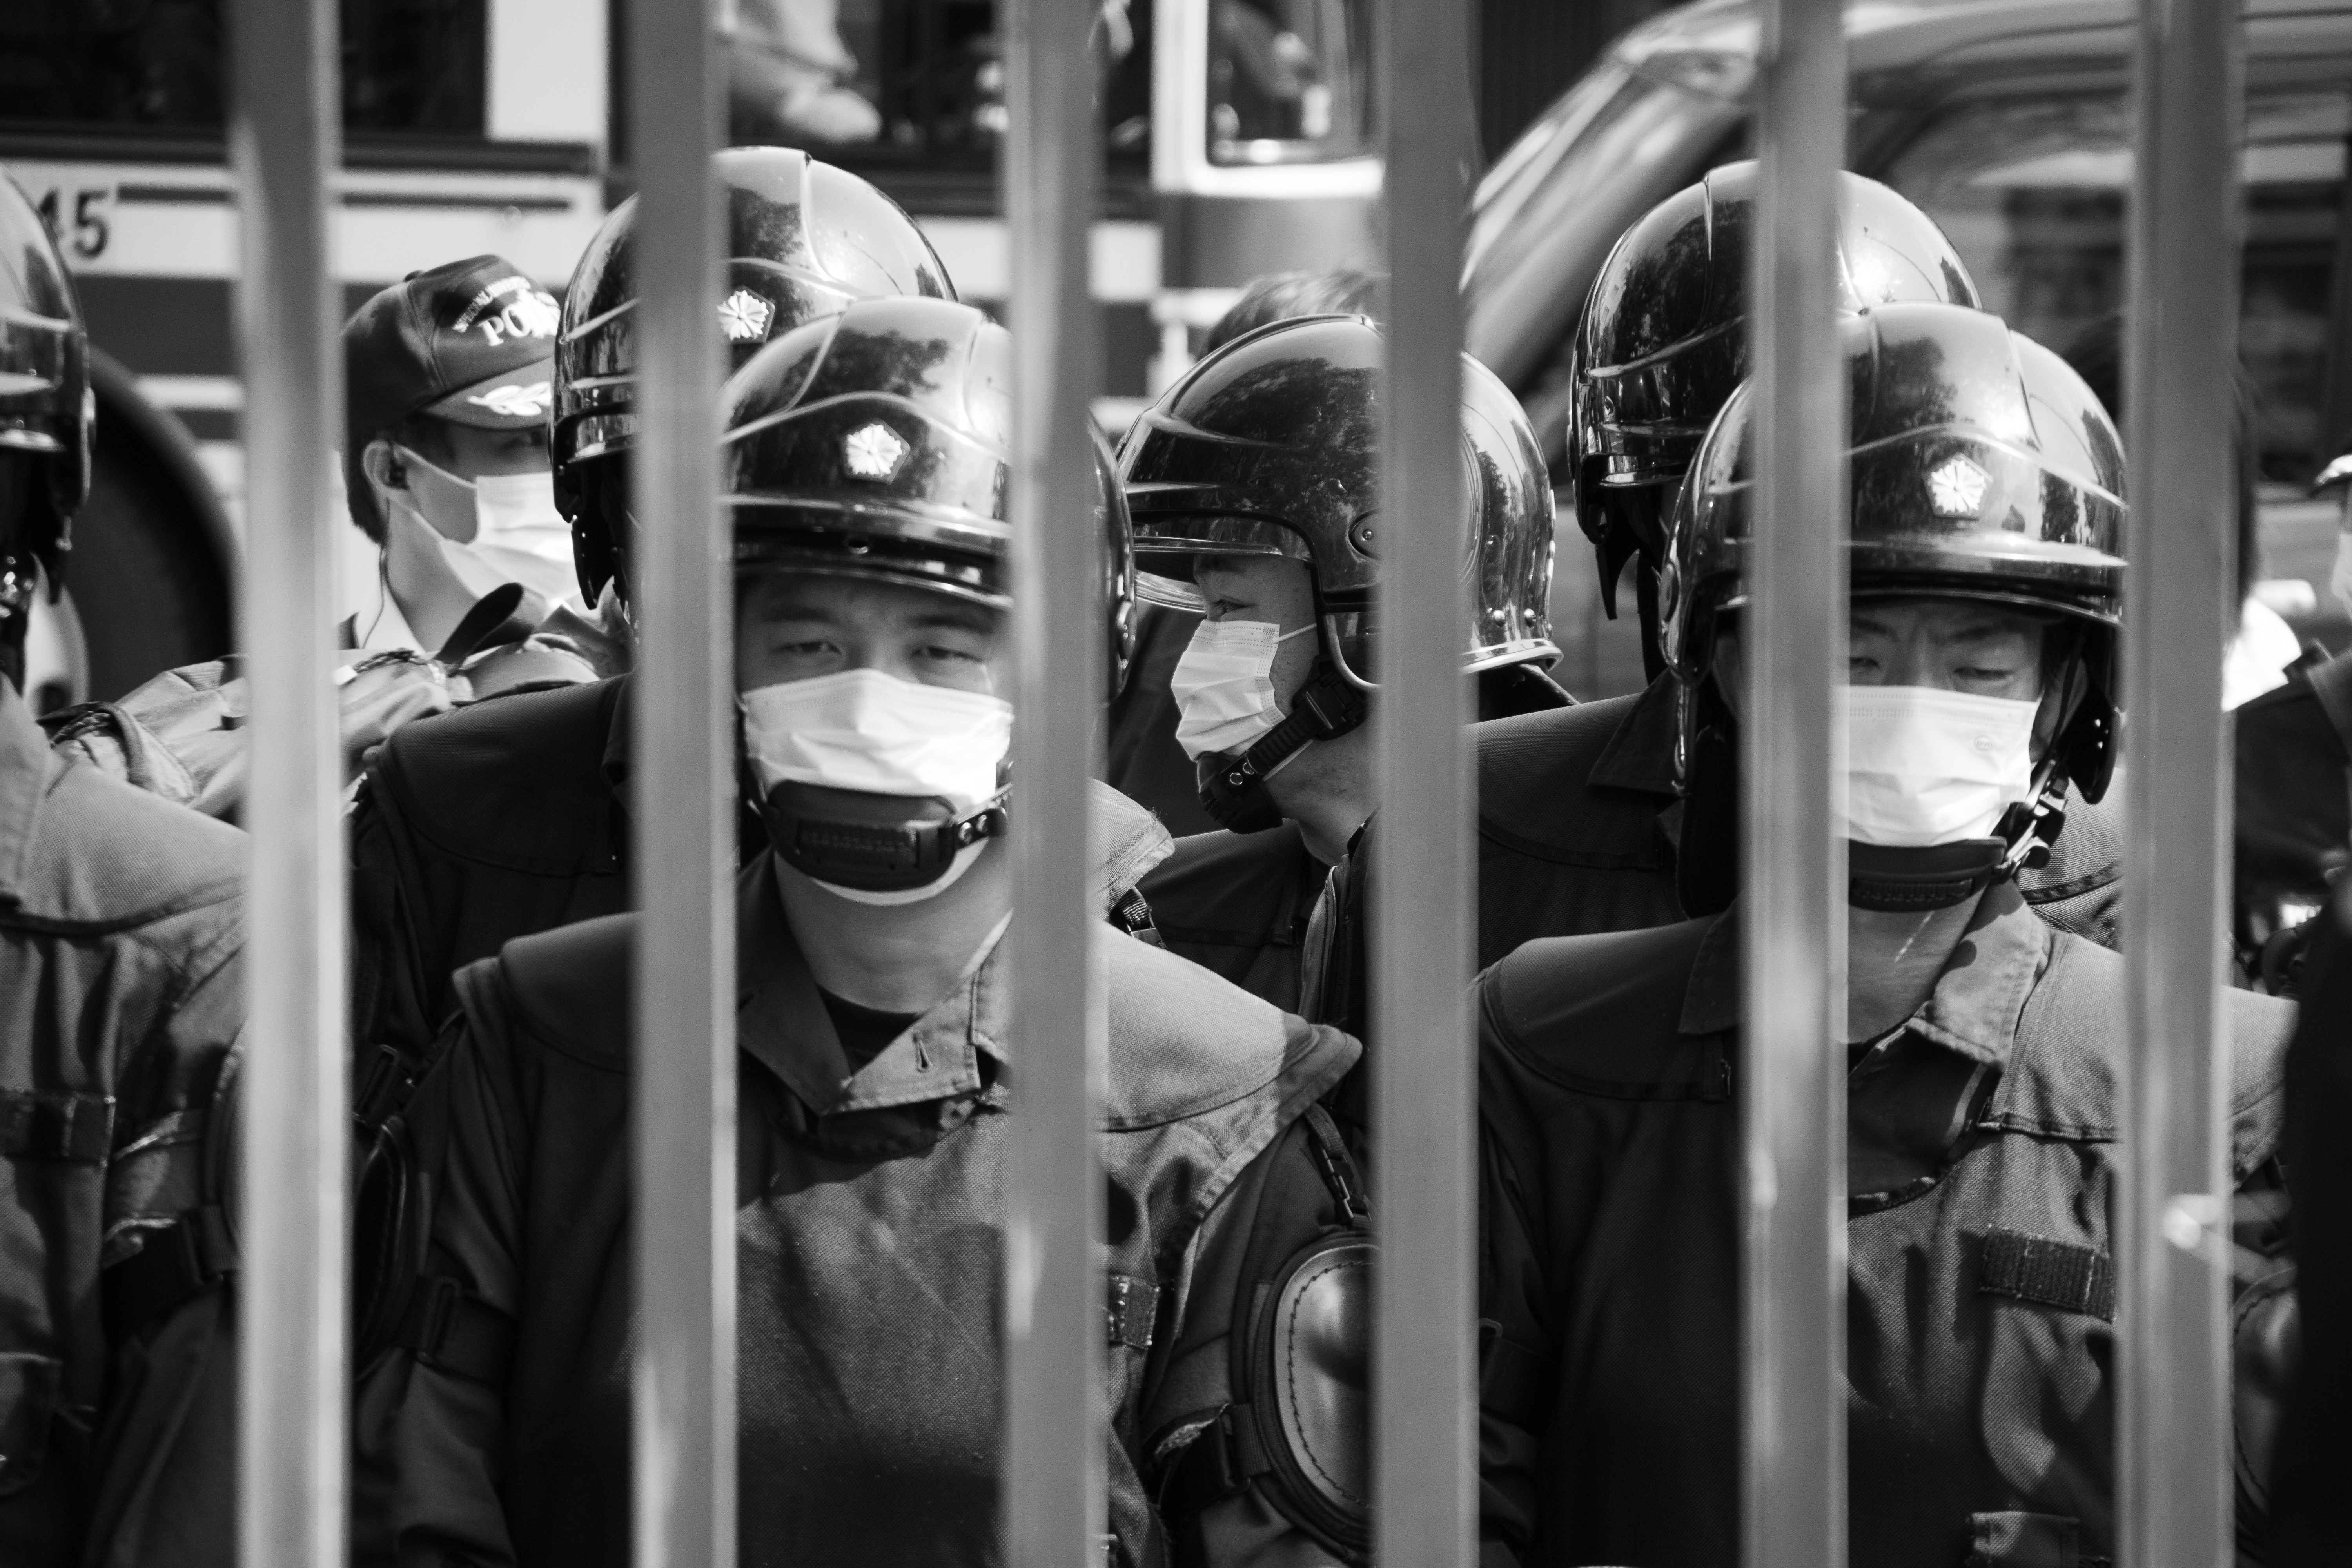
\includegraphics[width=5cm]{gazo/kidotai.jpg}
%   \caption*{{\small 封鎖された正門前に並ぶ機動隊}}
% \end{wrapfigure}

熊野寮は京大の敷地です。学問の自由を定めた憲法との関係から、警察のガサには京大職員の付添が必要です。なので、警察はガサの直前に京大に立ち入る旨の連絡をします(これは熊野寮以外の京大構内に立ち入る場合も同様です)。連絡を受けた大学は熊野寮自治会に対して直ちに捜索の連絡をいれる手筈になっています。

今回の場合は8時45分ころに寮に当局から電話があったので、その時点で熊野寮の正門を封鎖し、正門周辺に寮生がサングラスなどで顔を隠して集合しました。目的は機動隊の寮内雪崩込み占領とどさくさに紛れての令状不提示を防ぐためでした。しばらくすると立ち会いの大学職員と複数台のカメラと記者たちが門前に到着しました。今回もマスコミには警察からリークがあったようです。えろう仲がよろしおすなあ(京都弁)。

\begin{wrapfigure}[10]{o}[1cm]{6cm}
  \centering
  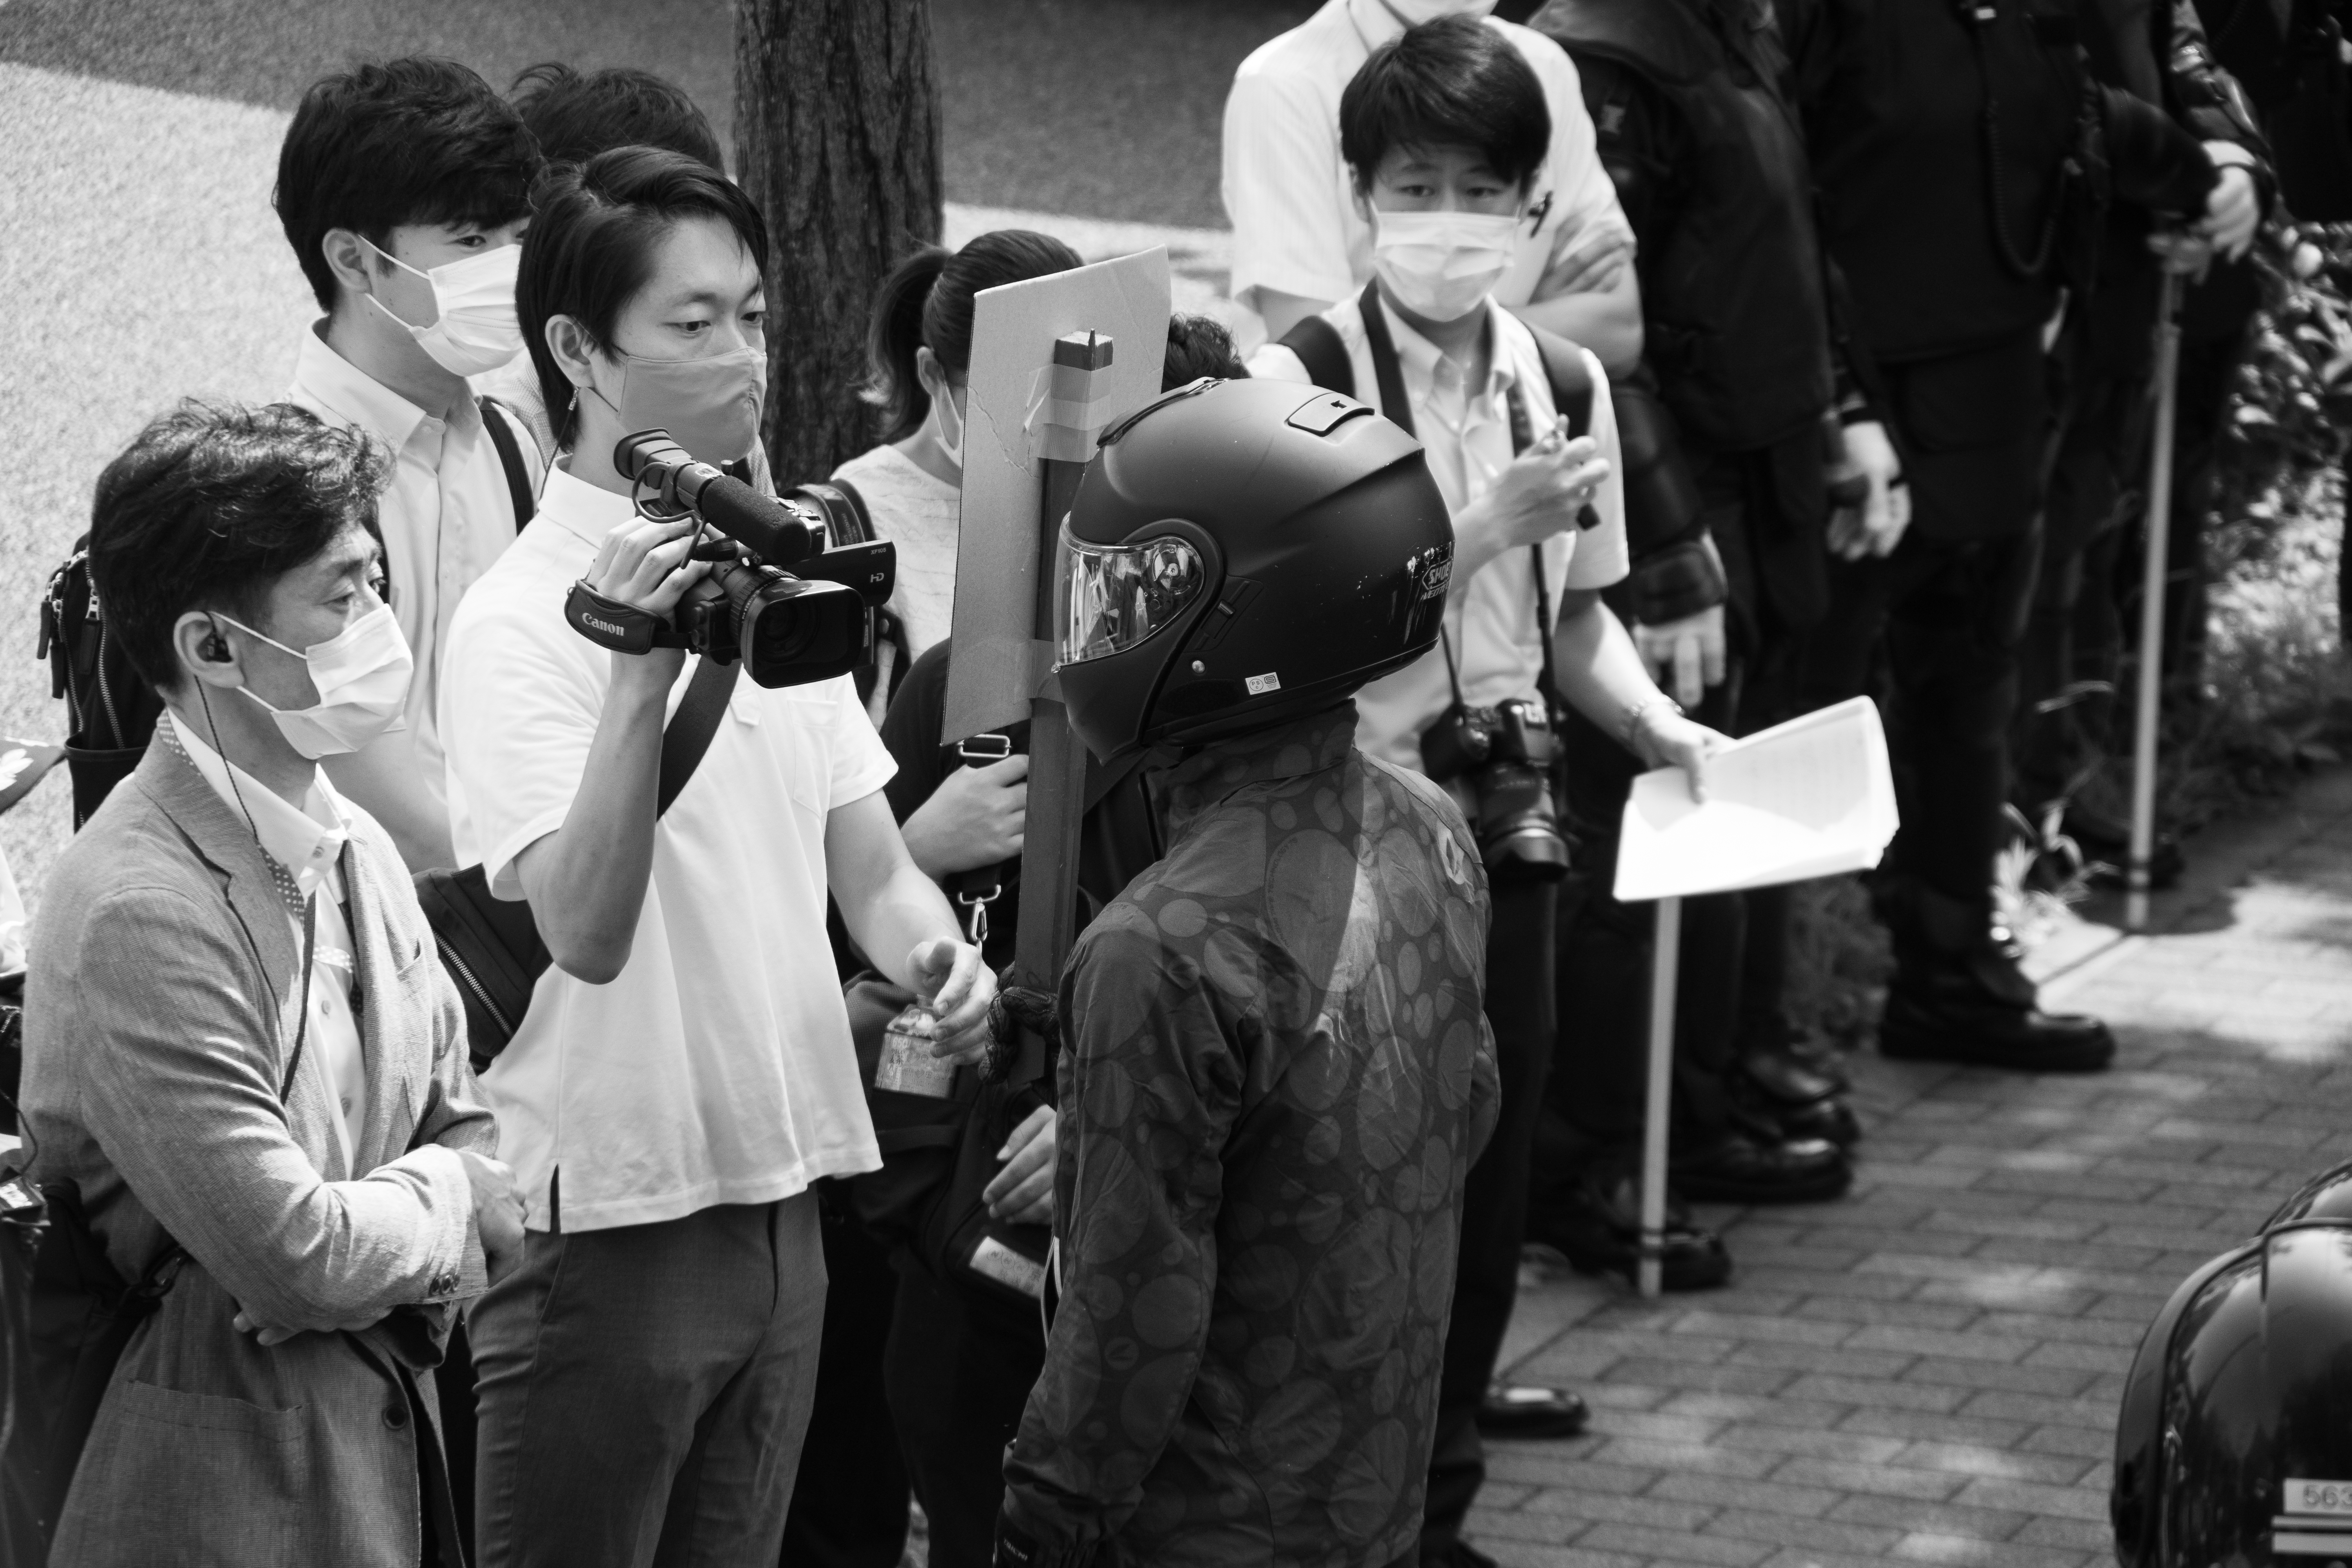
\includegraphics[width=5cm]{gazo/media.jpg}
  \caption*{{\small メディアと対峙。数年前には「顔を隠しているのは全て過激派」などという根拠のない報道があった。覆面をするのはプライバシーを守るため}}
\end{wrapfigure}

捜査員が大量(報道によると200名らしい)の機動隊を引き連れてやってきたのは9時ころでした。「かまぼこ」と呼ばれる護送車が寮の前に停止すると、警棒で武装した機動隊がぞろぞろと降りてきました。先頭には武装はしていないが強面の公安捜査員。門の中で見ていた僕の感想は「あーこれが権力かあ」です。自分が住んでいる場所への明確な敵意とそれを執行するのに十分な武力動員。大人200人あまりが免状不実記載ごとき微罪に動員されたという事実。ちょっと怖かったですが、寮生もそれなりに集まりましたし、何よりこっちには憲法や刑事訴訟法がついているので、心強くもありました。熊野寮門前は途端に機動隊で埋め尽くされましたが、こちらの意図通り無理やり寮内に侵入するということは阻止しました。


\begin{wrapfigure}[10]{o}[1cm]{6cm}
  \centering
  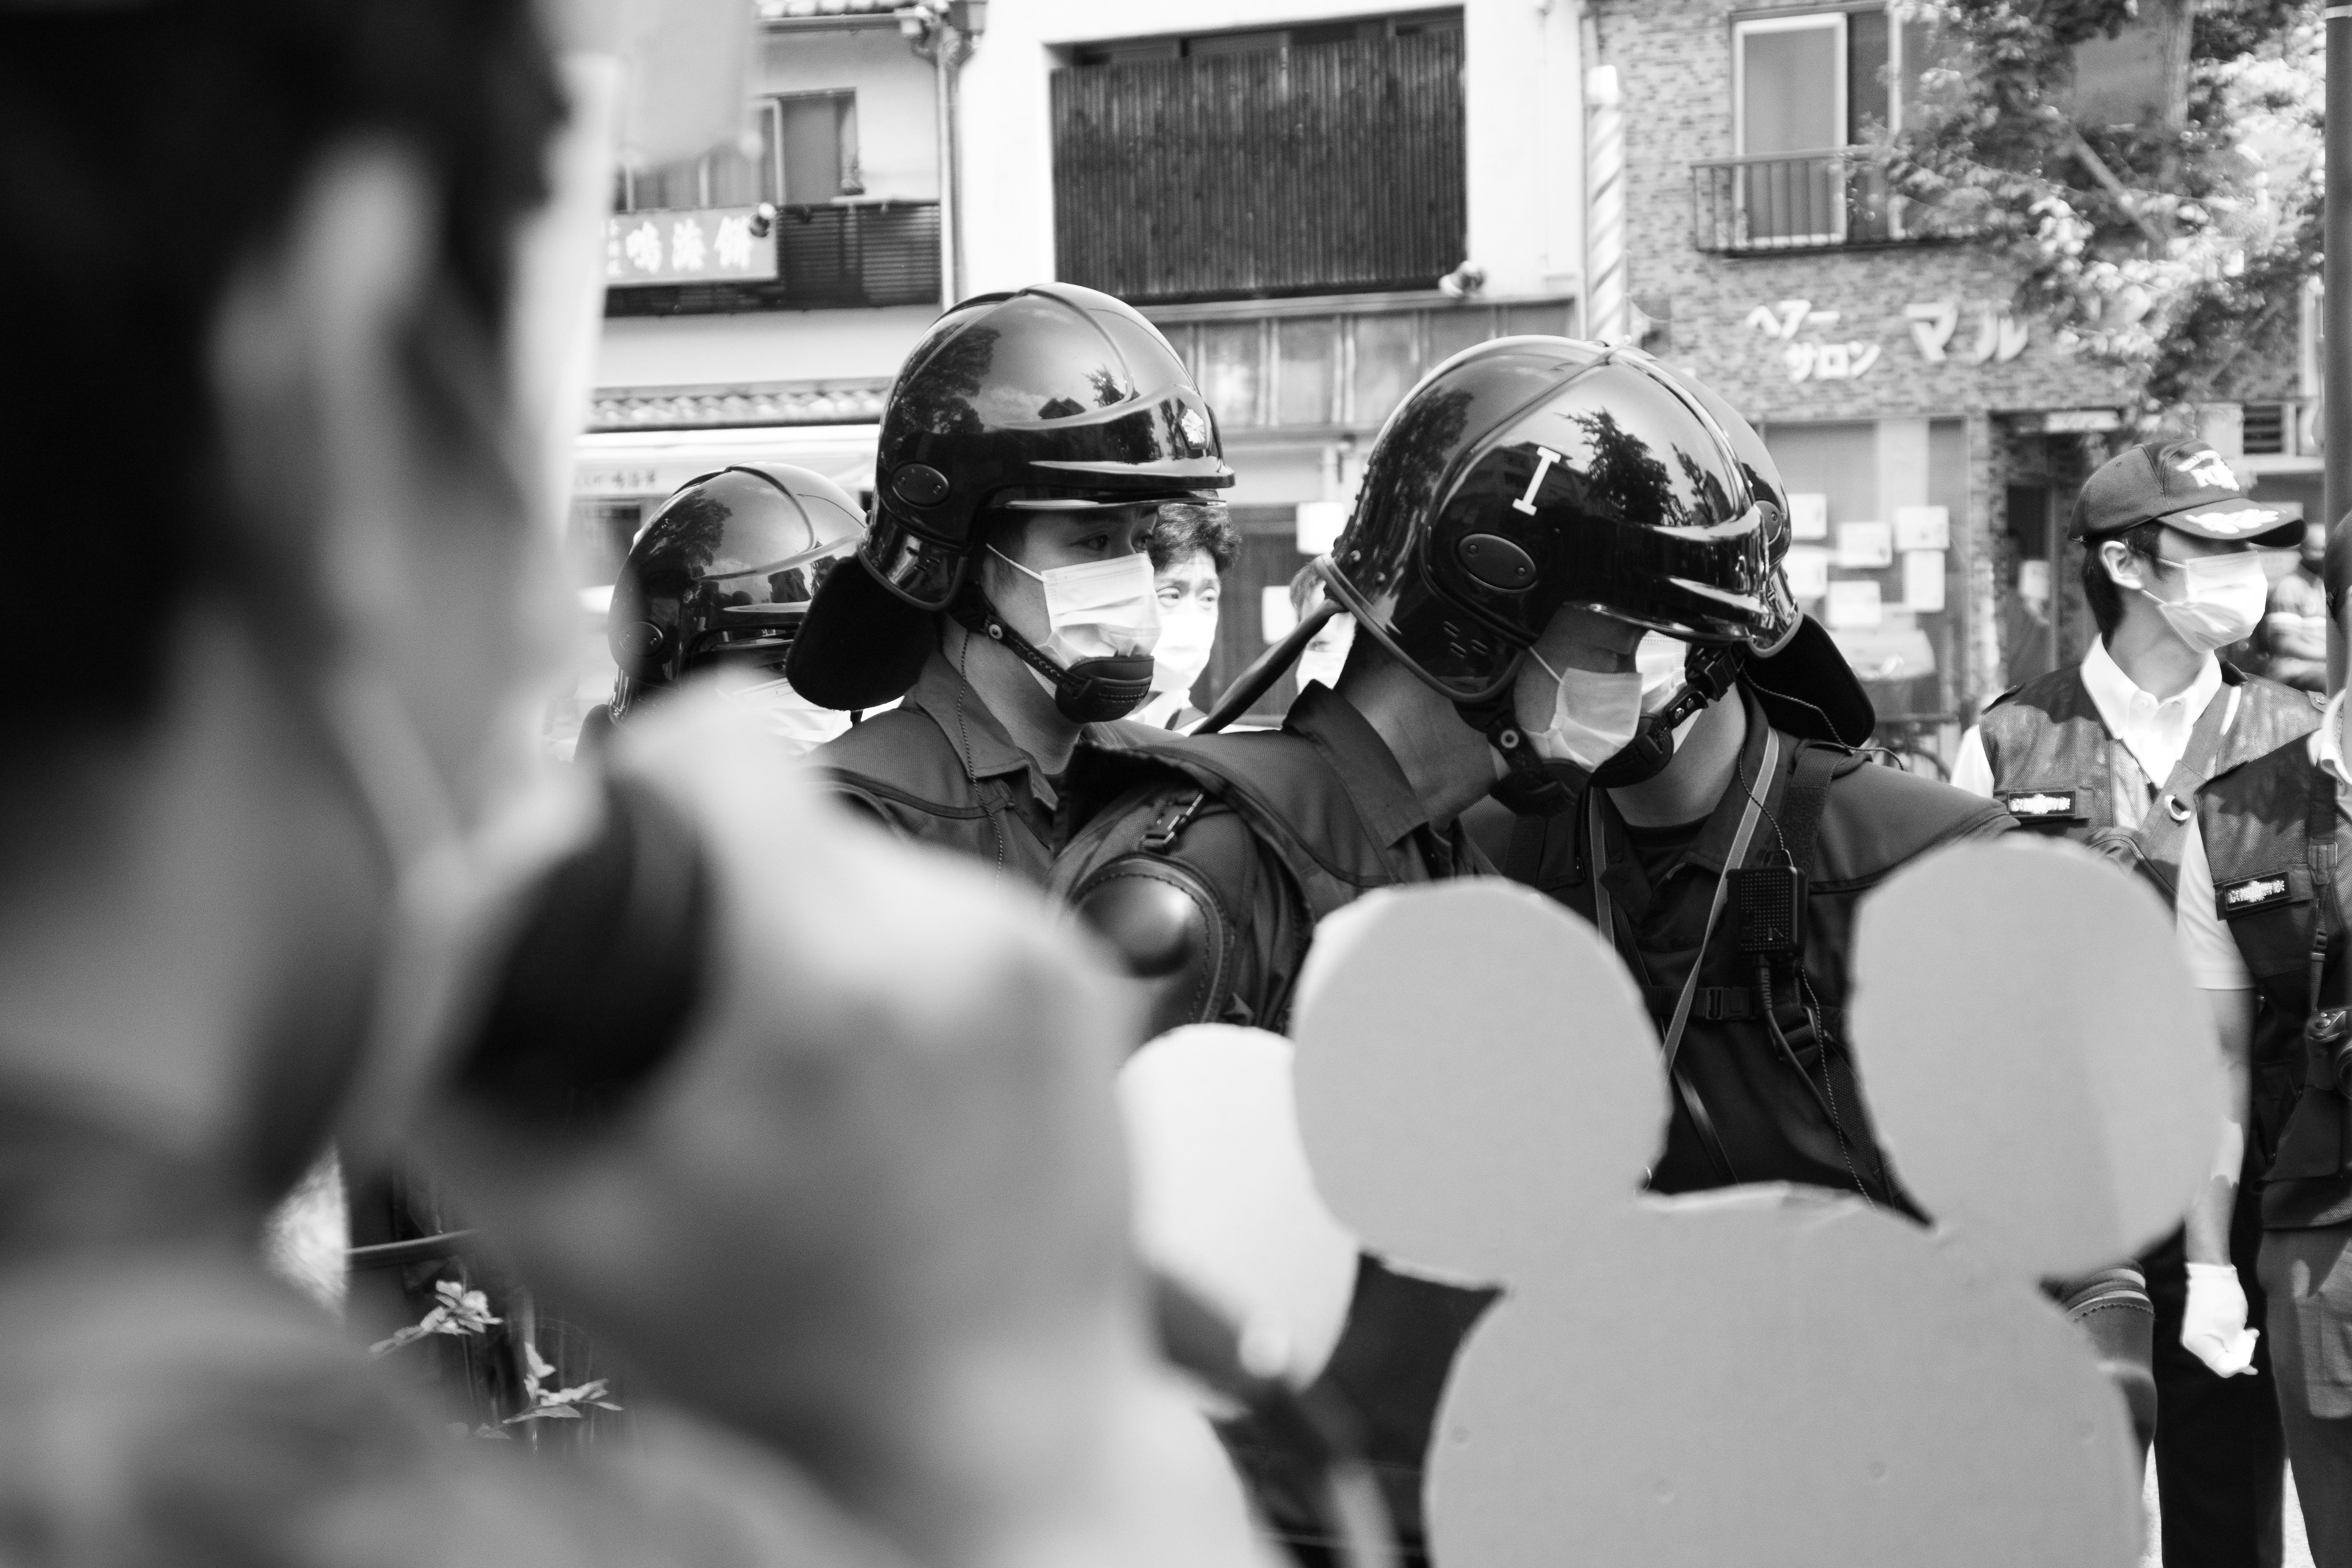
\includegraphics[width=5cm]{gazo/mikki.jpg}
  \caption*{{\small 声が通らないので拡声器を使って交渉。ミッキーのお面も活躍。}}
\end{wrapfigure}

\subsubsection{令状を見せて下さい}




さて、ここから交渉が始まります。まずは令状を見せるように言いました。それに対して捜査員は「捜索立会人(部屋等の捜索にあたっては、その部屋の住民などの立ち会いが必要)に見せる」という趣旨の主張をしてきました。しかし、寮内に立ち入るにも関わらず、寮生に令状を見せないということが許されるのでしょうか(本当に令状を持っているかわからない警察を寮内に入れることは当然できません)。そこでこちらは「法令に則って、ここで呈示して下さい」と反論すると、捜査員は「ここで議論はしない」と叫び、「捜査妨害するんですか」と威圧してきました。こっちも絶対に公務執行妨害で逮捕されたくないので「令状を確認すれば捜査には協力する。法令に則って令状を呈示してください」とメディアにも聞こえるように必死に叫びました。

\begin{wrapfigure}[10]{o}[1cm]{6cm}
  \centering
  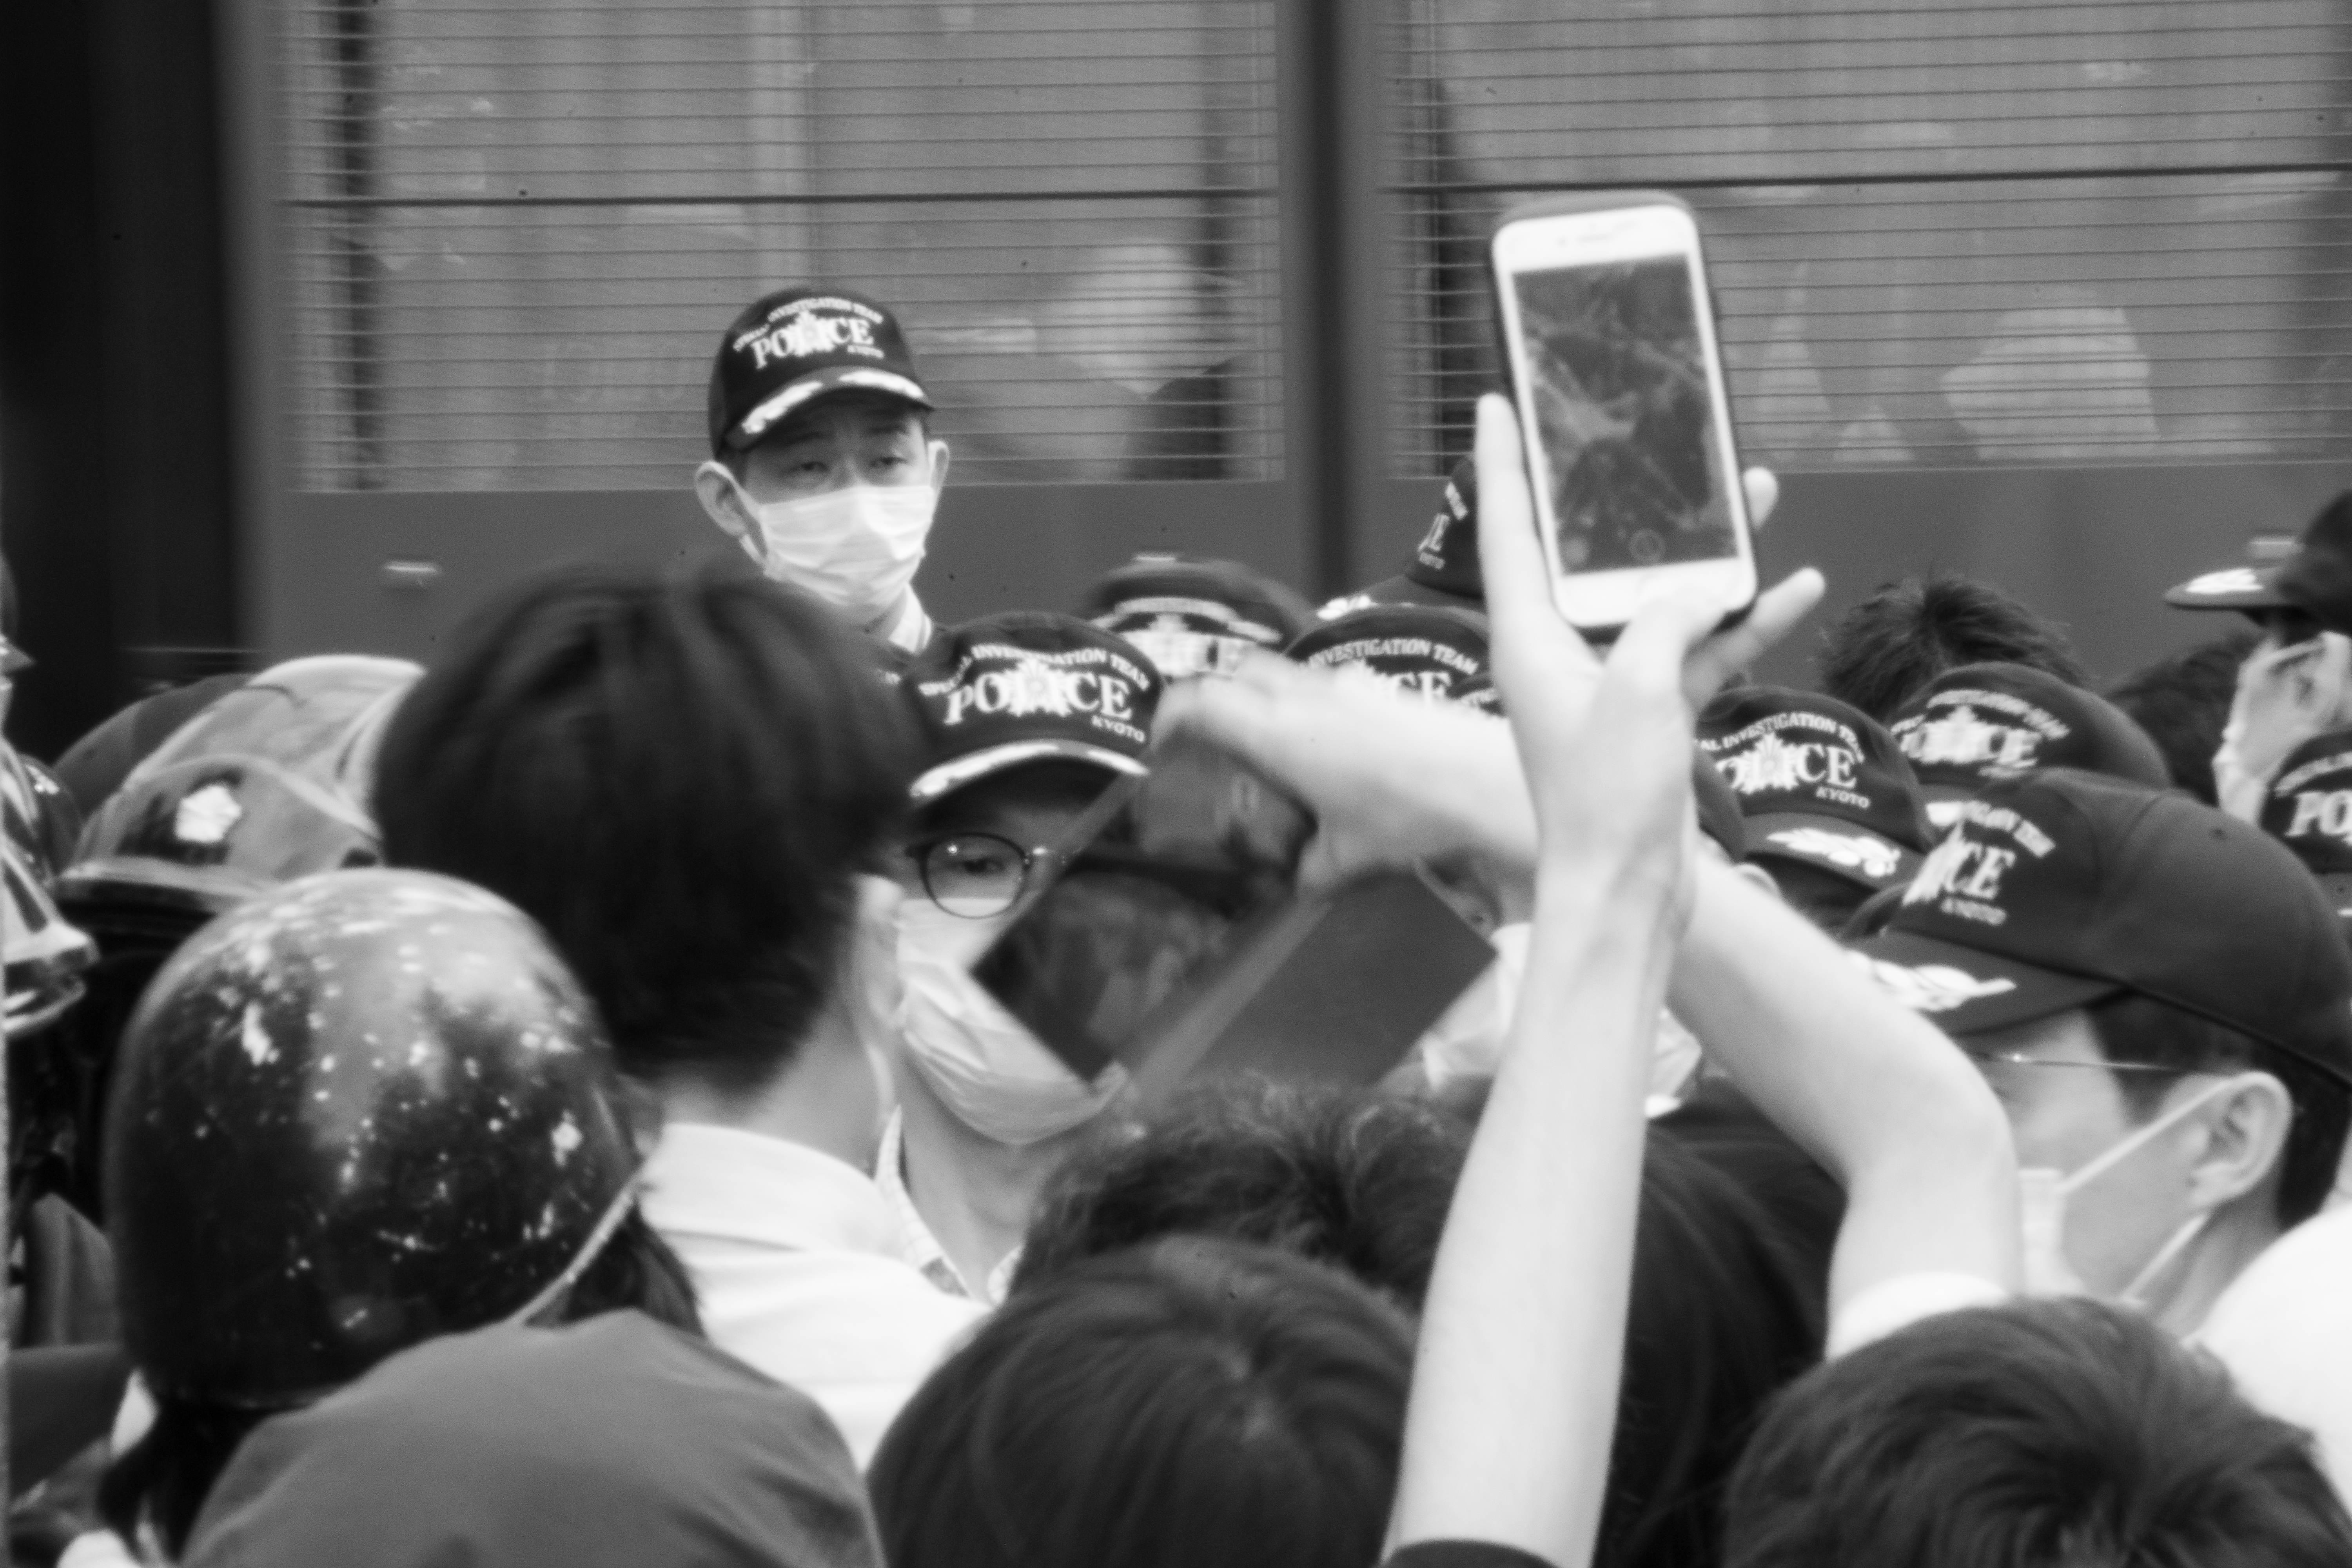
\includegraphics[width=5cm]{gazo/rejo_yomiage.jpg}
  \caption*{{\small 令状読み上げのシーン。警察は令状を撮影されることを拒んだ(背景の車が「かまぼこ」)}}
\end{wrapfigure}


2,3分押し問答した結果、令状は呈示され京大職員と寮生で読み上げました(ただし、捜査員がしっかりと見せてくれなかったので読み上げは不十分でした)。法的根拠なく令状の呈示を渋っていたとすれば、「警察やば」案件ですね。




\subsubsection{機動隊は入らないで下さい}

「令状見せてもろたし、ほな案内しまひょ」とはならないですね。捜査に機動隊は必要ないですから。捜査をするのはあくまで武装してない捜査員です。機動隊は過去に法的根拠なく寮内の廊下や階段を占拠したことがあるのは前述の通りです。つまり邪魔。こちらとしては、機動隊を寮内に入れる訳にはいきません。「捜査に協力するので機動隊を引かせて下さい」と主張すると「それはこっちで判断する」。「ここでは交渉しない。君らがこんな人数で妨害するから必要なんや」と叫ばれました。やっぱり逮捕されたくないので「あなた達が過剰警備をしているので抗議しているだけで妨害の意図はありません」と負けじと叫びます。

同様の押し問答のあと、寮生の主張が受け入れられました。\textbf{結局、機動隊は捜索の警備に必要なかったようですね}。機動隊員1人につき1万円の日当が支払われていたとすれば、少なくとも200万かかっている計算になります(ガバ計算)。僕たち寮生を脅したかったのか、それとも予算を消化したかったのか、どっちなんでしょうねえ。えらい仰山で来はって、賑やかどすなあ(京都弁)。


\subsubsection{令状のないプライバシー侵害}

捜索中にもやばい点がいくつかありました。僕が直接見たわけではなく、他の寮生から聞いたものですが、\textbf{捜索場所以外の部屋}の中を扉が開くたびに捜査員が覗き込んだり、駐輪場のバイクのナンバーをメモするなどしていたらしいです。令状はないので、ただのプライバシーの侵害です(当然、憲法・法令違反)。やばいですね。


\subsubsection{押収品について}

さて、寮内に入らなかったとは言え、200人もの機動隊を動員して行われたこの大規模な捜査で何か見つかったのでしょうか。捜索を受けたのは2箇所です。ここに2通の文書があります。
\begin{figure}[h]
  \begin{minipage}{0.5\textwidth}
    \centering
    \includegraphics[width=8cm]{gazo/oushuhinmokuroku.jpg}
    \caption*{{\small 押収品目録}}
  \end{minipage}
  \begin{minipage}{0.5\textwidth}
    \centering
    \includegraphics[width=8cm]{gazo/sosakushomesho.jpg}
    \caption*{{\small 捜索証明書}}
  \end{minipage}
\end{figure}

それぞれの部屋でどんな証拠が押収されたのかを示す警察が発行した文書です。1つ目は押収物目録。押収されたのはノート一冊とあります。もう一つは捜索証明書。これは、押収物がなかったときに捜索がすでになされたということを証明するための文書で、日本でこれが発行されるのはかなりレアです。なぜなら証拠が確実に見つかる場合にしか捜索はされないからです。ネット上では刑事訴訟マニアによって高額での取引がされているとか、いないとか。

\textbf{つまり今回の捜索では、寮生の私物のノート一冊しか押収していないのです。}しかもこのノートの持ち主によると、Aさんの免状不実記載についての記述はこのノートにはないそうです。\textbf{さすがに手ぶらで帰るというのは警察のメンツ的にまずかったのでしょうか。}つくづくやばい組織ですね。

なお「400点もの押収品があった」というテレビ報道もありましたが、大嘘もいいところですね。警察とそんなに懇ろなんだったら嘘掴まされるなよ。お前らいいように使われてるだけやぞ。真実を報道しろ。ボケナス。

すいません。怒りが漏れてしまいました。


\subsection{ガサと寮生}

\begin{wrapfigure}[15]{o}[1cm]{4cm}
  \centering
  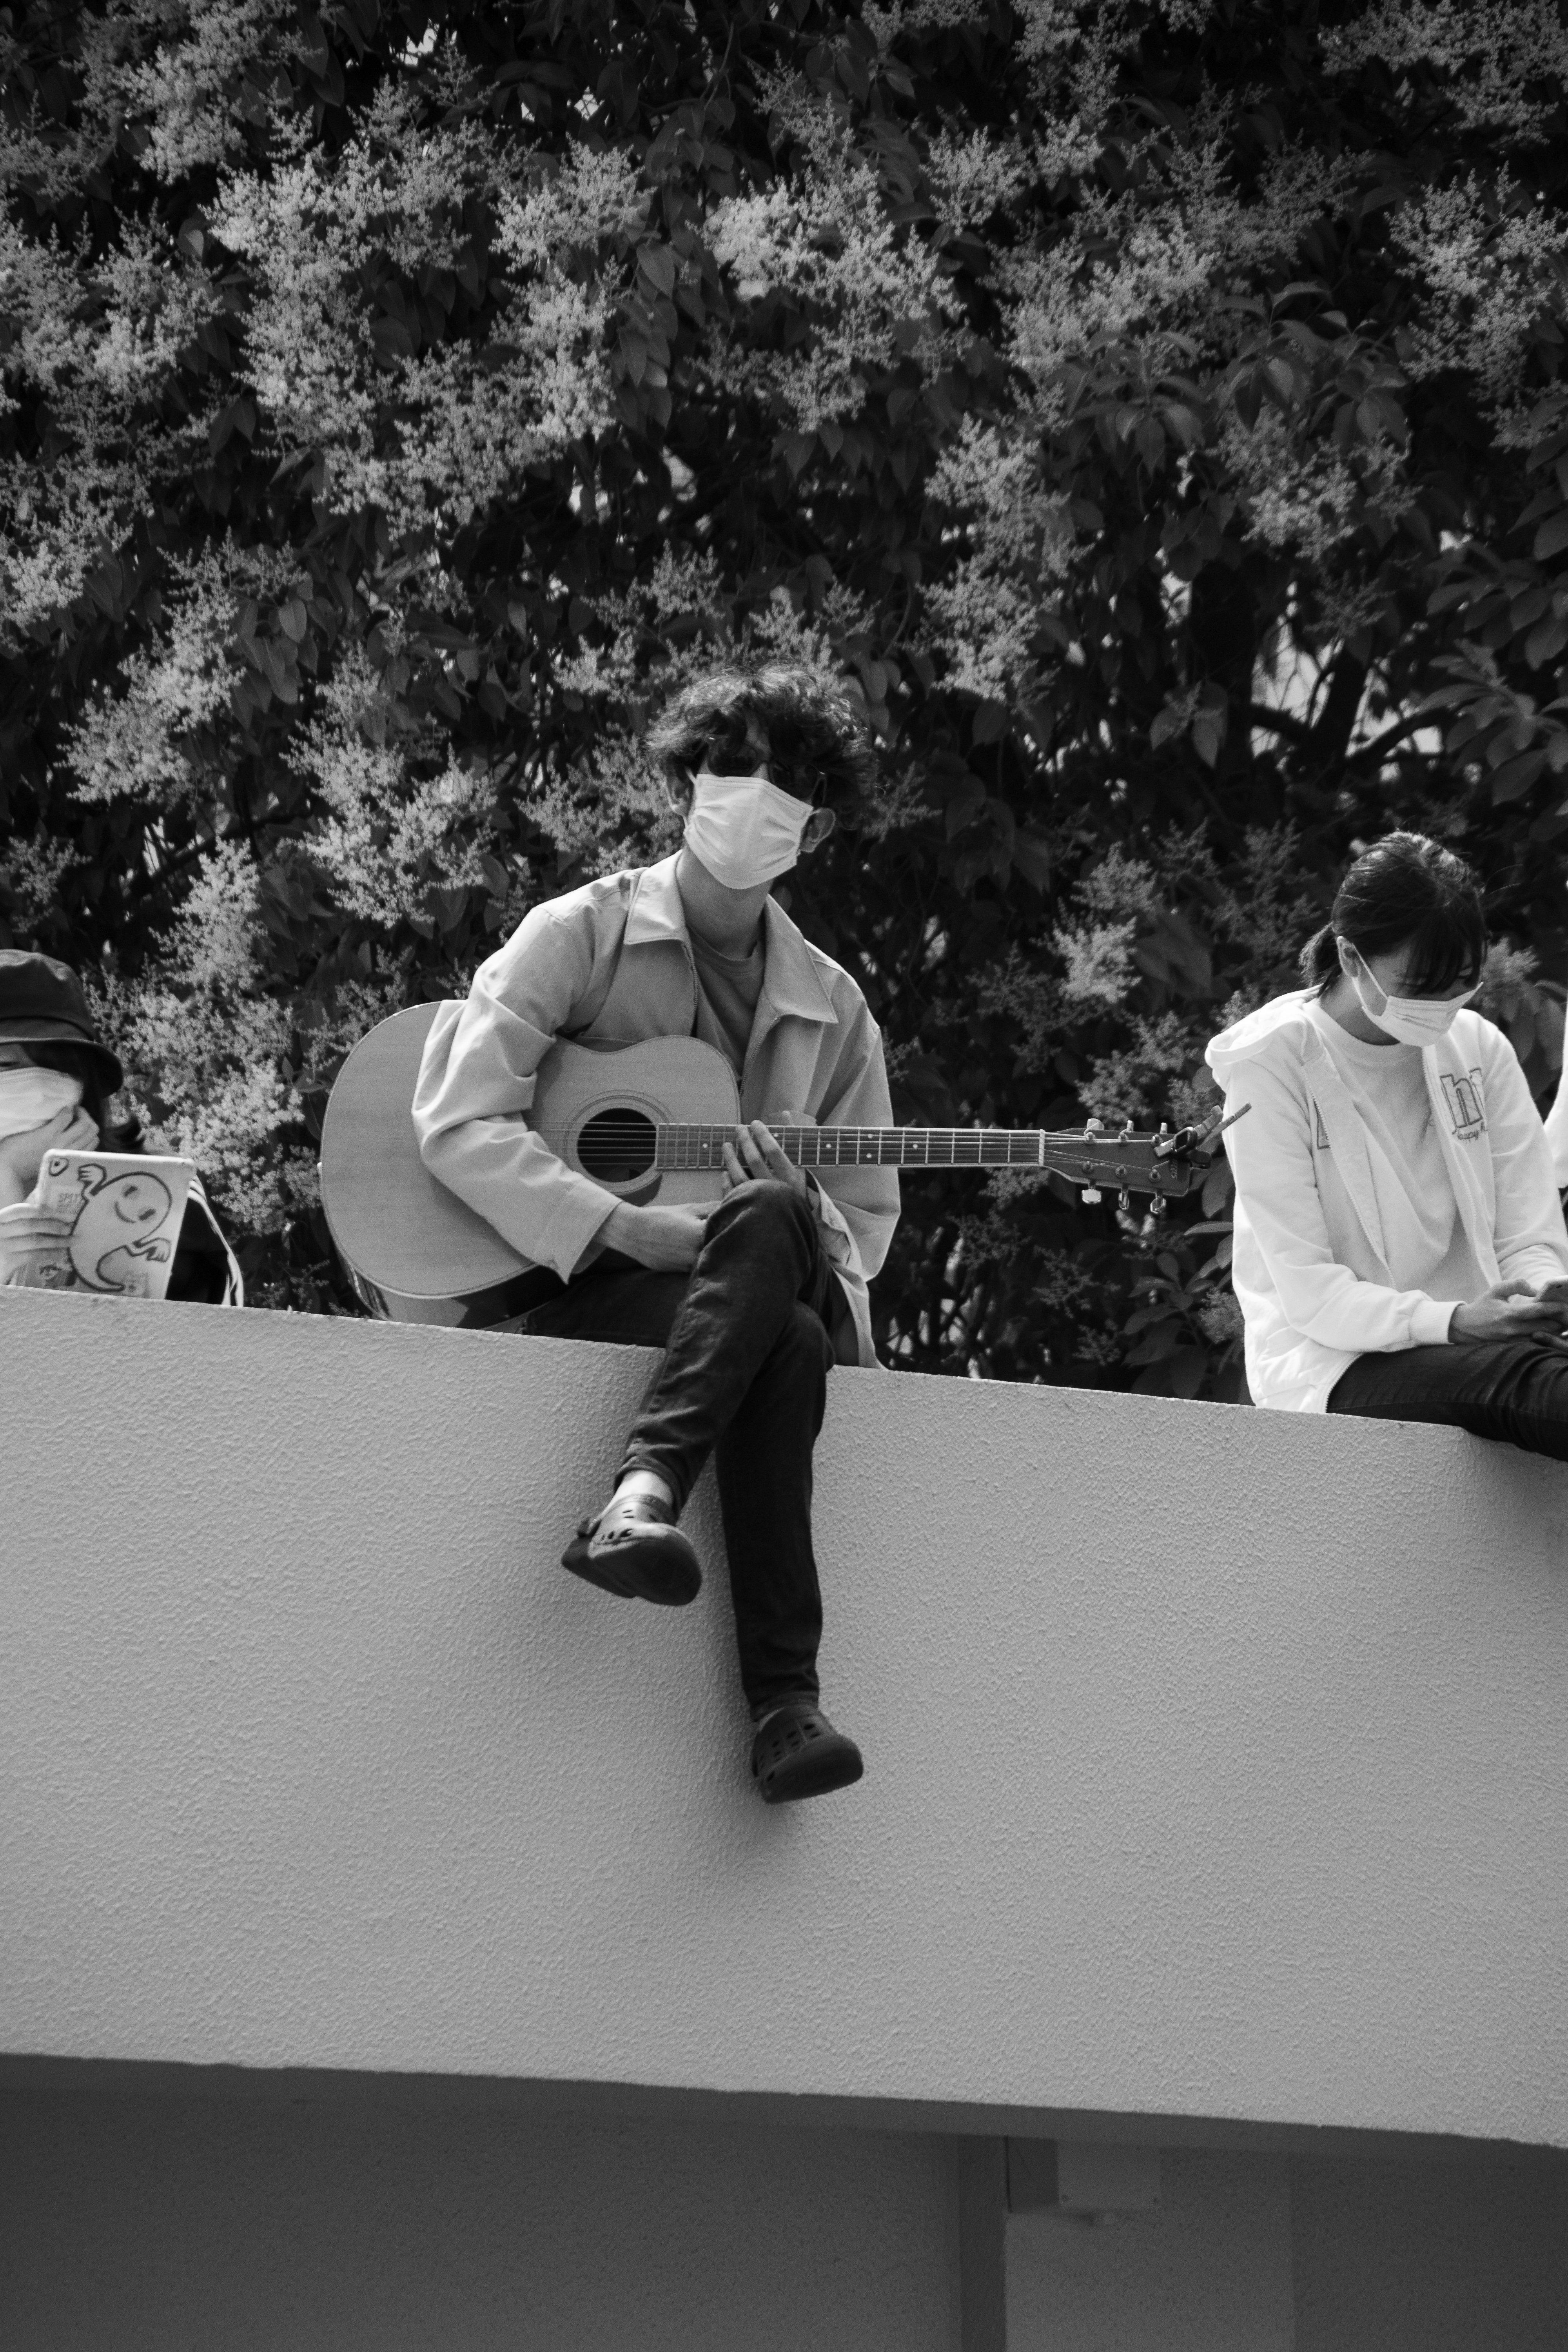
\includegraphics[width=3cm]{gazo/live.jpg}
  \caption*{緊急ライブ(演目はスピッツ「チェリー」など)}
\end{wrapfigure}

ガサが来た日は京大の授業日でした。機動隊の隣をすり抜けて大学に向かったり、授業には行かずに警察の対応や抗議をしたり、警察と世間話をしたり、メディアの撮影に抗議したり、報道カメラマンみたいに動き回って写真を撮影したり、屋上で眺めたり、ラブ\&ピースを訴えて緊急ライブをギター1本で開催したり、ガサには興味なく部屋にいたり、寮生はいろいろな仕方でガサの時間を過ごしました。僕は寮を守りたいという気持ちで正門前でずっと警察の対応をしていました。捜索の不当性や過去にあった違法な捜索の事例は寮内でだいたい共有されていると思いますが、ガサにどう向き合うかは個人に任されています。中には「ガサって楽しい」と思った寮生も多いと思います。不当な権力と、みんな一緒に法律(とミッキーのお面)片手に対峙することである種の興奮が生まれるのは当然です。僕もちょっぴり楽しかった。




けれど、忘れてはいけないのは、\textbf{今回の逮捕やガサは明白な人権侵害だということ}(上でも述べたとおりです)と、単純にガサが迷惑な人も多いということです。授業に普通に行きたかった人もいましたし、熊野寮のガサで友人や親から心配されたり、「熊野寮に住んでいるなんて危ない人だ」と偏見を持たれたりした人も多くいます。僕もやりましたが親への説明が結構面倒なんですね。この記事が親の説得に役立てばいいなあ。


\subsection{まとめ}

いかがでしたか。結局、警察が熊野寮に捜索に来た理由はわかりませんでした。

というのは嘘でおおかたの理由はわかります。\textbf{要は熊野寮のネガキャンです。}熊野寮は機動隊付きでガサが来るような場所ですよ、「やばい」場所ですよと、メディアまで動員して宣伝をしているわけです。寮外から見たら、実際そのように見えていたでしょう。でも寮の中から見たら、警察の方が遥かに「やばい」のです。その風景をみなさんと少しでも共有できればありがたいです。

\rightline{写真提供:みかみかみ(ツイッター\url{@mikamiormi})}

{\scriptsize この記事は、webサイト「千万遍石垣」に2021年10月12日に投稿した記事を修正したものです。}
